\chapter{考察}\label{cha:Discussion}
本研究では、電子フォーム作成時間の削減を目的としたラベル付き記入欄検出手法の提案を行った。
本提案手法は、以下に示す2つの機能を持つ。

\begin{itemize}
  \item ラベル付き領域座標取得機能
  \item 領域描画画像出力機能
\end{itemize}

5章では、本提案手法が持つ2つの機能について、正しく動作することを確認した。
本章では、まず、本提案手法の有用性について考察する。次に、本提案手法と関連研究を比較する。最後に、本提案手法の問題点について述べる。

\section{本提案手法の有用性に関する評価}\label{sec:evalue_usefulness}
本提案手法の有用性を評価するため、本提案手法を、電子フォーム作成ツールであるPhotolizeに適用し、実験を行う。
Photolizeは、スマートフォンで撮影した帳票の画像に対して、電子フォーム記入欄を配置することによって、電子フォームを作成するサービスである\cite{Photolize}。
本提案手法をPhotolizeに適用することで、帳票画像記入欄を検出し、領域座標とラベルをまとめたJSONファイルから、電子フォーム記入欄を配置する手間と時間を削減することができる。

実験は、2枚の帳票画像に対して本提案手法を適用し、検出できなかった帳票画像記入欄や、誤検出によって電子フォーム記入欄に対して、被験者には、Photolizeを利用し、電子フォーム記入欄を配置してもらう。
実験の対象とした帳票の画像を、図\ref{fig:experiment_A}と図\ref{fig:experiment_B}に示す。
図\ref{fig:experiment_A}は、本提案手法が入力の対象とする帳票画像のうち、電子文書の画像であり、図\ref{fig:experiment_B}は、電子化文書の画像である。
以降、図\ref{fig:experiment_A}の画像を、帳票画像A、図\ref{fig:experiment_B}の画像を、帳票画像Bと呼ぶ。

\begin{figure}[t]
    \begin{center}
        \fbox{
            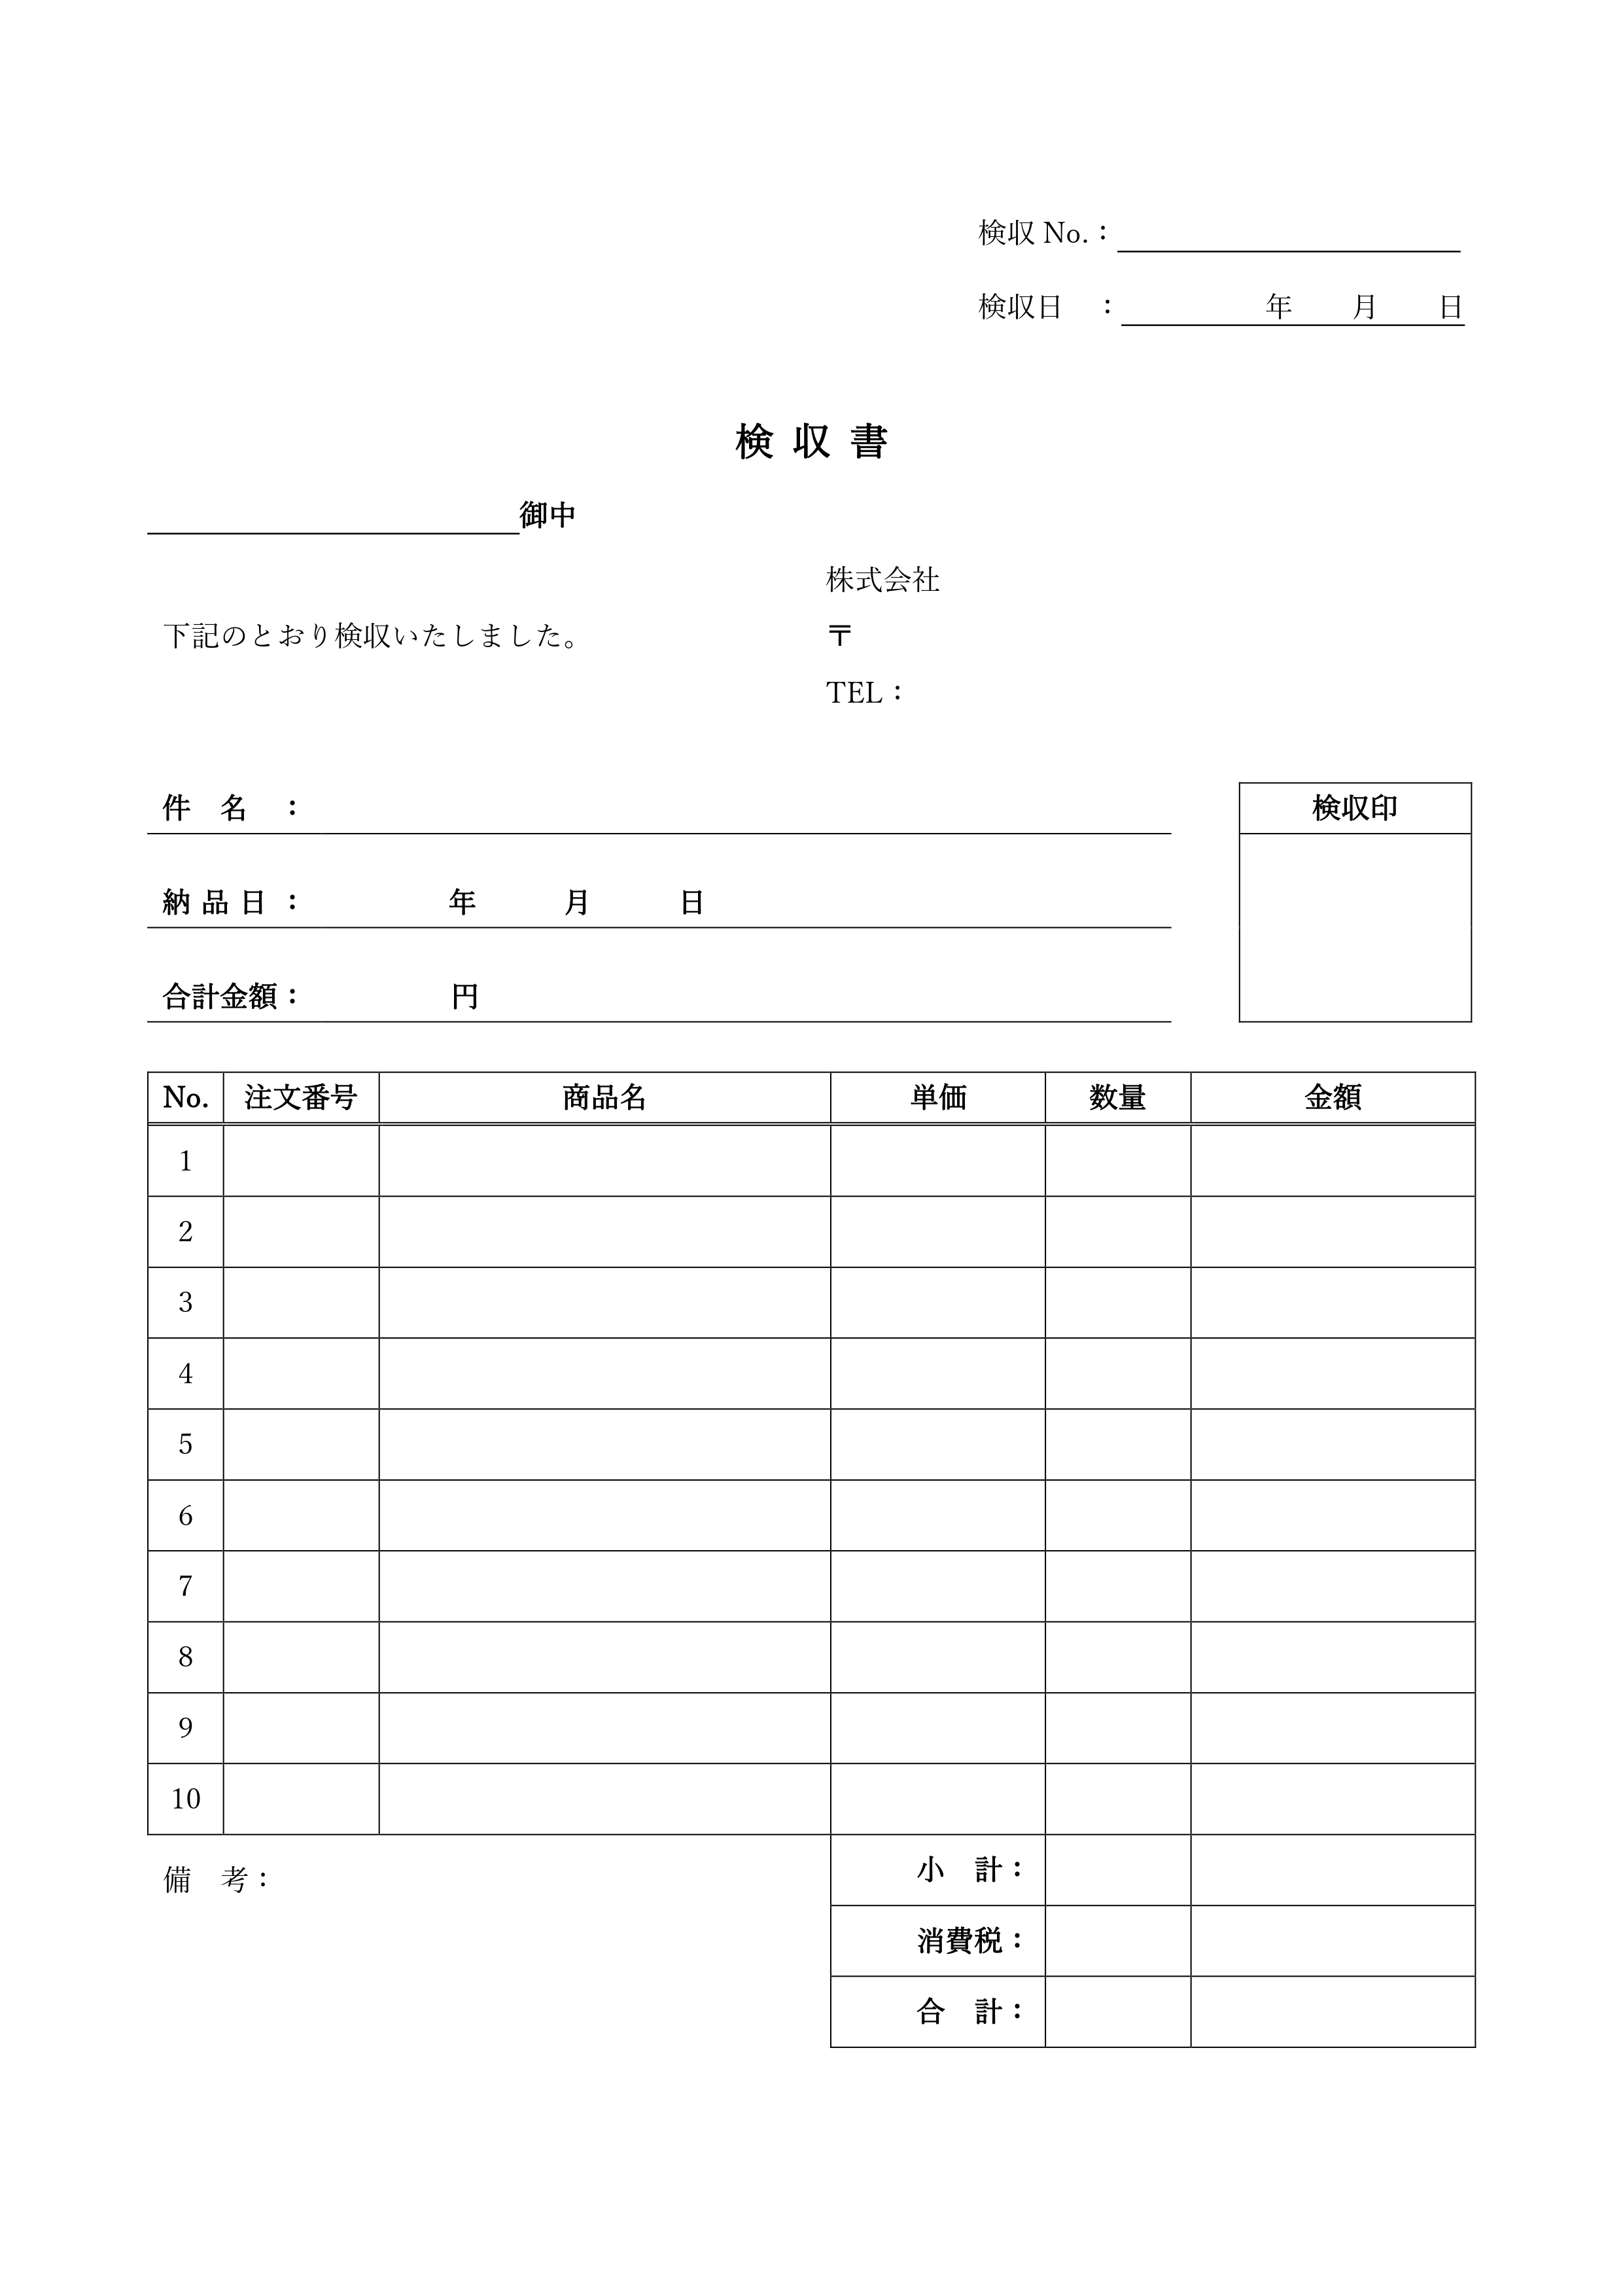
\includegraphics[width=15cm]{image/06-discussion/experiment_A.jpg}
            }
        \caption{実験対象である帳票画像A}
        \label{fig:experiment_A}
    \end{center}
\end{figure}

\begin{figure}[t]
    \begin{center}
        \fbox{
            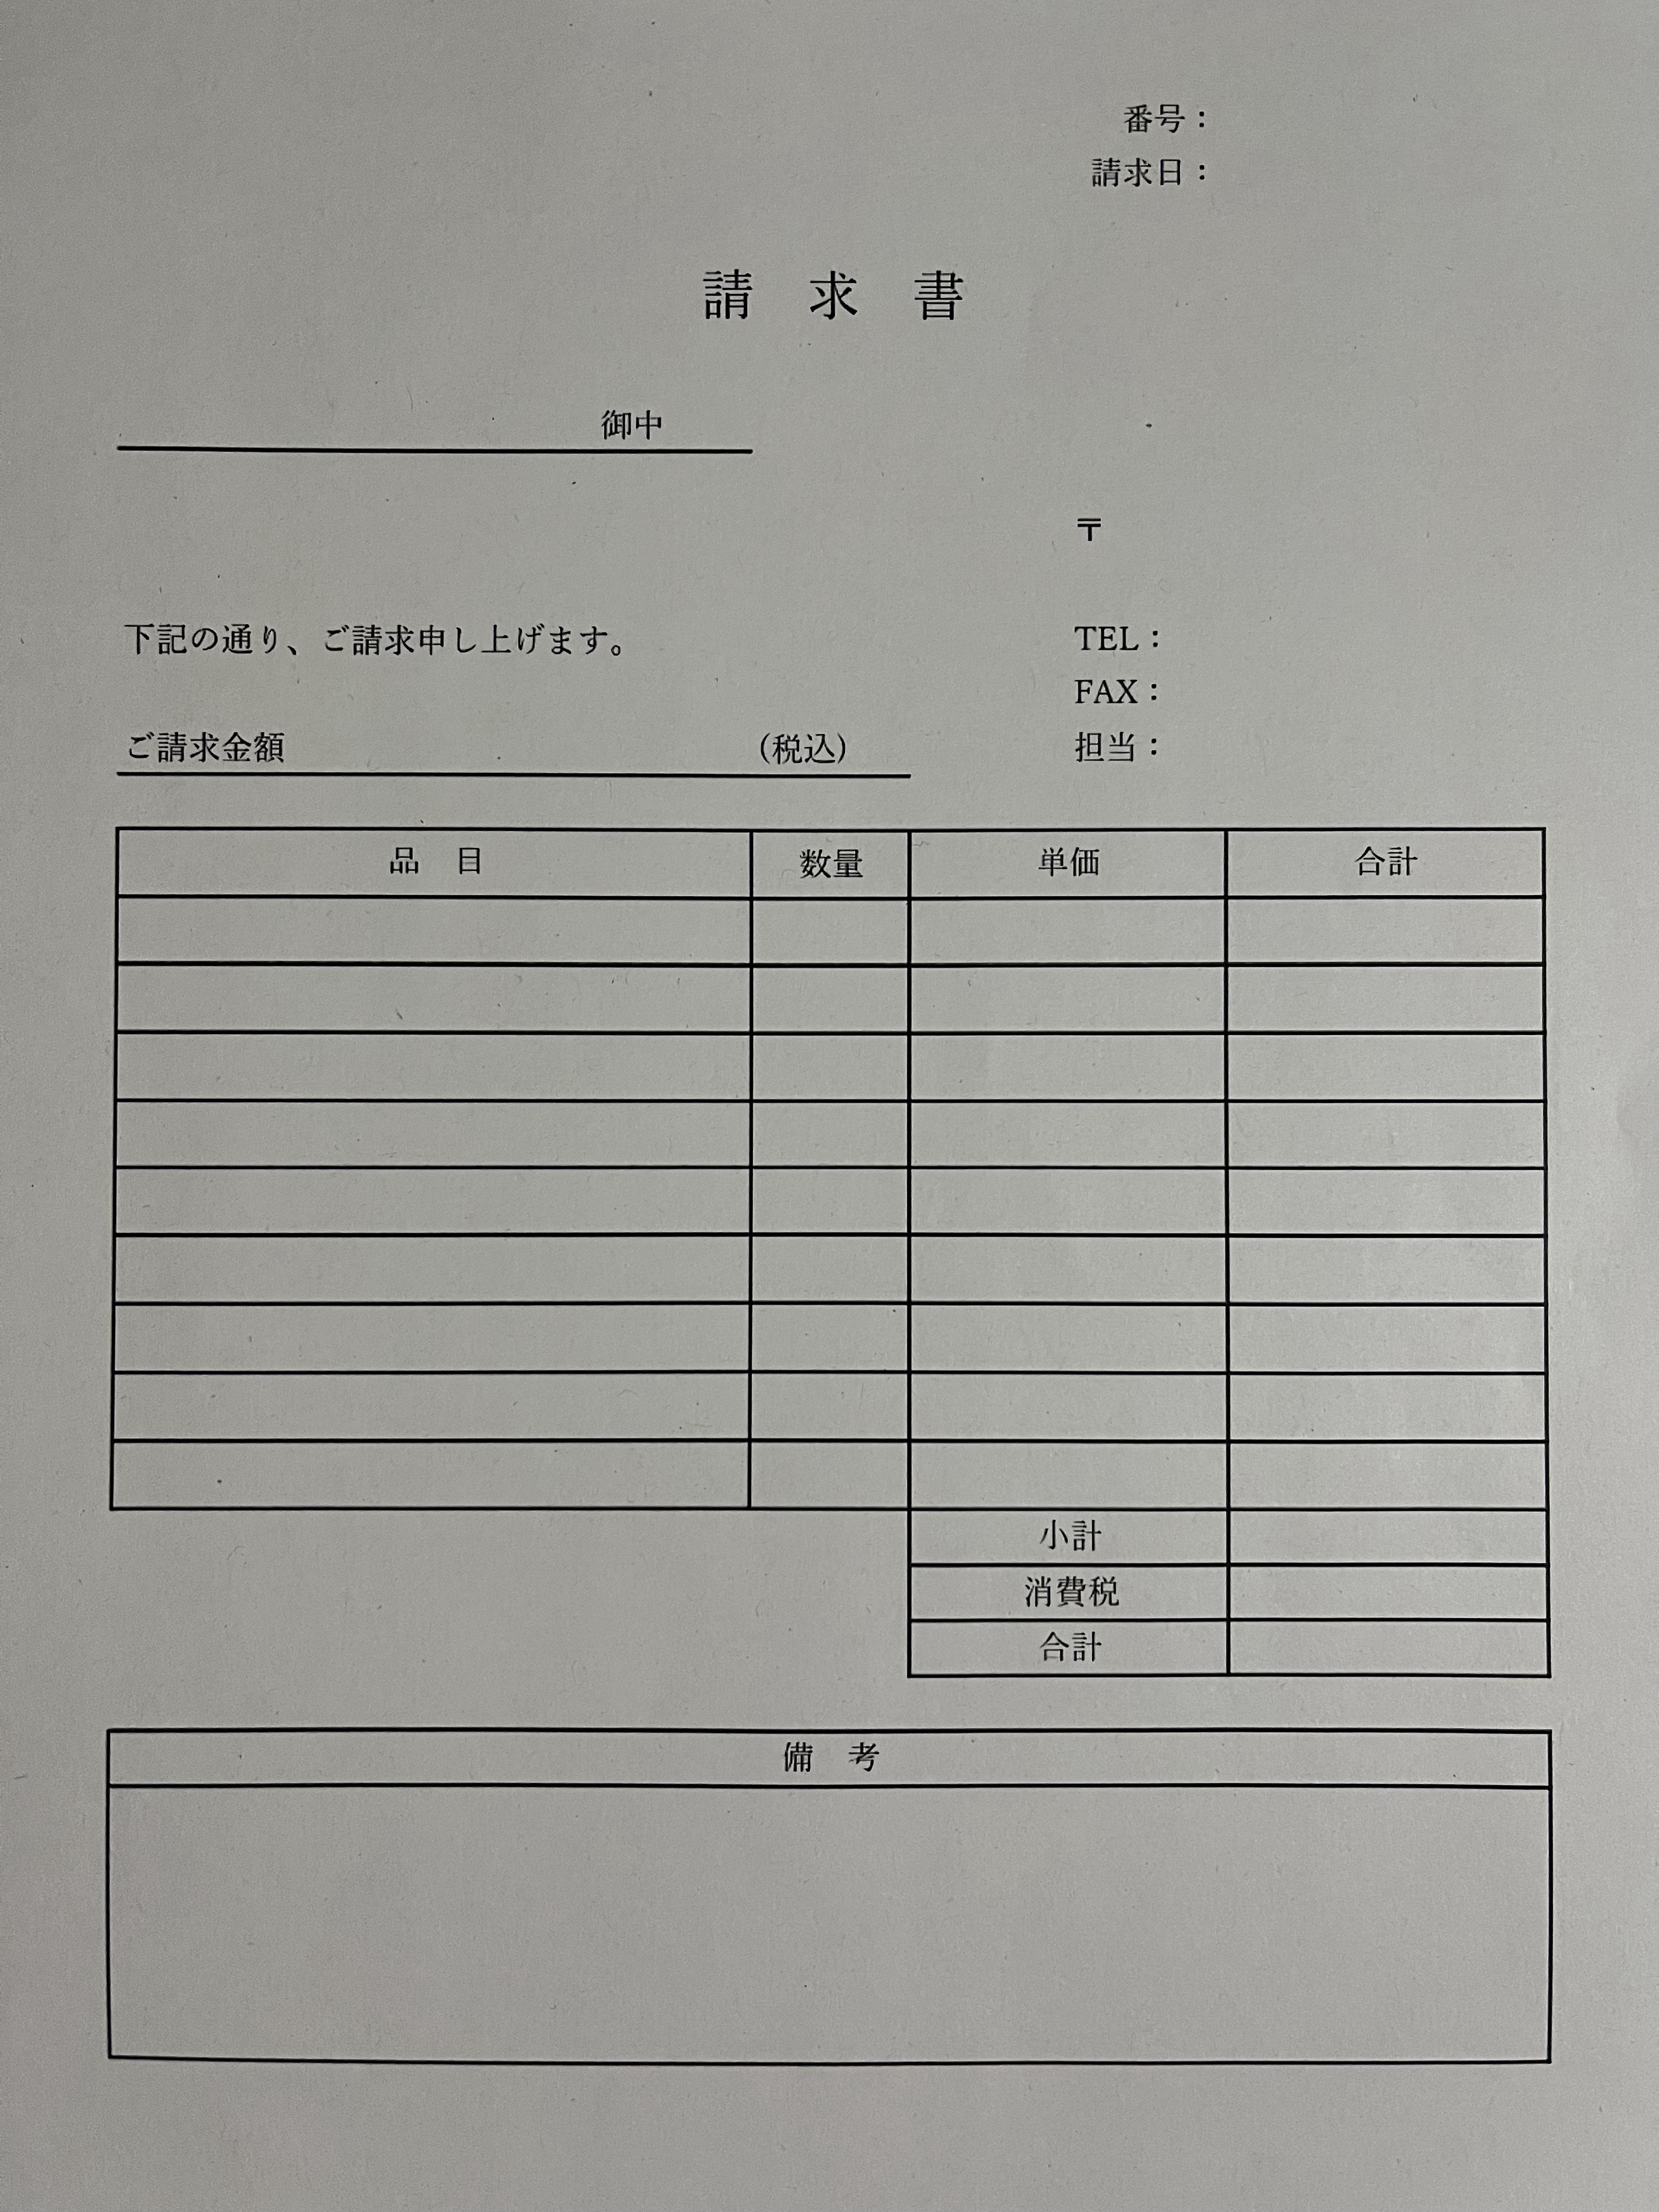
\includegraphics[width=15cm]{image/06-discussion/experiment_B.jpg}
        }
        \caption{実験対象である帳票画像B}
        \label{fig:experiment_B}
    \end{center}
\end{figure}

実験は、宮崎大学工学部情報システム工学科に所属する学部4年生X名、および修士1年生Y名、2年生Z名の計A名を対象として行った。

実験方法は、被験者A名を2つのグループに分け、片方のグループにケースAの実験を行い、もう片方のグループにケースBの実験を行う。
ケースAでは、図\ref{fig:experiment_A}の帳票画像に対して、本提案手法を適用せず、手作業で電子フォーム記入欄を配置してもらう。
次に、図\ref{fig:experiment_B}の帳票画像に対して、本提案手法を適用し、修正対象の電子フォーム記入欄を修正し、電子フォーム記入欄を配置してもらう。
ケースBでは、図\ref{fig:experiment_A}の帳票画像に対して、本提案手法を適用し、修正対象の電子フォーム記入欄を修正し、電子フォーム記入欄を配置してもらう。
次に、図\ref{fig:experiment_B}の帳票画像に対して、本提案手法を適用せず、手作業で電子フォーム記入欄を配置してもらう。

被験者が行った実験のケースを、以下の表\ref{tb:experiment_case}に示す。


\begin{table}[t]
	\centering
	\caption{被験者が行った実験ケースと手法}
    \label{tb:experiment_case}
    \begin{tabular}{cc}
        \begin{minipage}[c]{0.5\hsize}
            \centering
            \begin{tabular}{c|c}
                ケース & 被験者 \\
                \hline \hline
                \multirow{4}{*}{ケースA} & 被験者A \\
                                        & 被験者B \\
                                        & 被験者C \\
                                        & 被験者D \\
                                        \hline
                \multirow{4}{*}{ケースB} & 被験者E \\
                                        & 被験者F \\
                                        & 被験者G \\
                                        & 被験者H
	        \end{tabular}
        \end{minipage} &
        \begin{minipage}[c]{0.5\hsize}
            \centering
            \begin{tabular}{c|c|c}
                ケース & 帳票画像 & 手法 \\
                \hline \hline
                \multirow{2}{*}{ケースA} & 帳票画像A & 手作業のみ \\
                                        & 帳票画像B & 提案手法 + 修正 \\
                                        \hline
                \multirow{2}{*}{ケースB} & 帳票画像A & 提案手法 + 修正 \\
                                        & 帳票画像B & 手作業のみ
            \end{tabular}
        \end{minipage}
    \end{tabular}
\end{table}

なお、本提案手法で取得した領域座標、および、ラベルについては、間違っている可能性がある。
修正対象の電子フォーム記入欄に該当する電子フォーム記入欄を、以下に示す。

\begin{itemize}
    \item 誤検出によって、帳票画像内に帳票記入欄が存在しない場所に配置したもの。
    \item 帳票画像内に存在する帳票記入欄を検出できず、配置できていないもの。
    \item 本来想定するラベルとは異なるラベルを割り付けたもの。
\end{itemize}

実験で計測する時間について、本提案手法を適用し、JSONファイルと2枚の領域強調画像を出力するまでの時間を、実行時間と呼ぶ。
また、電子フォーム記入欄の配置が完了するまでの時間を、配置時間と呼ぶ。

実験の手順を、以下に示す。
なお、配置が必要な電子フォーム記入欄の数は、図\ref{fig:experiment_A}が54個、図\ref{fig:experiment_B}が48個である。

\begin{enumerate}
    \item 開始前に、実験対象の帳票画像とPhotolizeについて説明し、Photolizeにおける電子フォーム記入欄の配置操作も併せて説明する。
    \item 本提案手法を適用する場合は、実行時間を計測する。
    \item 適したラベルを考慮しつつ、電子フォーム記入欄の配置と修正をしてもらい、配置時間を計測する。
    \item 全電子フォーム記入欄の位置とラベルを確認し、正しく配置した割合を計算する。
\end{enumerate}



\subsection{電子フォーム記入欄の配置完了までにかかる時間に関する評価}\label{subsec:evalue_required_time}
本節では、電子フォーム記入欄の配置完了にかかる時間について、評価を行う。
実験結果のうち、各計測時間とその平均をまとめたものを、表\ref{tb:result_time}に示す。
また、合計時間を算出する式を、式\ref{eq:sum_time}に示す。
なお、手作業のみで枠を配置した場合は、実行時間は0秒として計算する。

\begin{equation}\label{eq:sum_time}
    合計時間=実行時間+配置時間
\end{equation}

表\ref{tb:result_time}より、帳票画像Aに関する合計時間は、ケースAがケースBよりも平均でX分Y秒(約Z\%)短い。
同様に、帳票画像Bに関する合計時間は、ケースBがケースAよりも平均でX分Y秒(約Z\%)短い。
以上の結果から、本提案手法は、電子フォーム記入欄を配置する時間の削減について、有用であることがわかった。

% \begin{table}[t]
% 	\caption{被験者が配置完了までにかかる時間}
% 	\label{tb:result_time}
% 	\centering
% 	\begin{tabular}{ccc||rrrr|r}
% 		被験者 & ケース & 帳票画像 & 実行時間 & 配置時間 & 合計時間 \\
%         \hline \hline

% 		% 宮下さん M2
% 		\multirow{2}{*}{被験者A} & \multirow{2}{*}{ケースA} & 帳票画像A & 00:00 & 08:49 & 08:49 \\
% 		                        &                          & 帳票画像B & 01:10 & 03:49 & 04:59 \\
%                                                            \hline

% 		% 
% 		\multirow{2}{*}{被験者B} & \multirow{2}{*}{ケースA} & 帳票画像A & 00:00 &  &  \\
%                                 &                          & 帳票画像B &  &  &  \\
%                                                            \hline

% 		%
% 		\multirow{2}{*}{被験者C} & \multirow{2}{*}{ケースA} & 帳票画像A &  &  &  \\
%                                 &                          & 帳票画像B &  &  &  \\
%                                                            \hline

% 		%
% 		\multirow{2}{*}{被験者D} & \multirow{2}{*}{ケースA} & 帳票画像A & 00:00 &  &  \\
%                                 &                          & 帳票画像B &  &  &  \\
%                                                            \hline

% 		%
% 		\multirow{2}{*}{被験者E} & \multirow{2}{*}{ケースB} & 帳票画像A &  &  &  \\
%                                 &                          & 帳票画像B & 00:00 &  &  \\
%                                                            \hline

% 		%
% 		\multirow{2}{*}{被験者F} & \multirow{2}{*}{ケースB} & 帳票画像A &  &  &  \\
%                                 &                          & 帳票画像B & 00:00 &  &  \\
%                                                            \hline
% 		%
% 		\multirow{2}{*}{被験者G} & \multirow{2}{*}{ケースB} & 帳票画像A &  &  &  \\
%                                 &                          & 帳票画像B & 00:00 &  &  \\
%                                                             \hline
% 		%
% 		\multirow{2}{*}{被験者H} & \multirow{2}{*}{ケースB} & 帳票画像A &  &  &  \\
%                                 &                          & 帳票画像B & 00:00 &  &  \\
%                                                             \hline
% 		\hline \hline
% 		% 平均
% 		\multirow{4}{*}{平均}  & \multirow{2}{*}{ケースA} & 帳票画像A & 00:00 &  &  \\
%                                &                         & 帳票画像B &  &  &  \\
%                                & \multirow{2}{*}{ケースB} & 帳票画像A &  &  &  \\
%                                &                          & 帳票画像B & 00:00 &  &  \\
% 	\end{tabular}
% \end{table}

\begin{table}[t]
	\caption{ケースAの被験者が配置完了までにかかる時間}
	\label{tb:result_accuracy}
	\centering
	\begin{tabular}{cc||rrrr|r}
		被験者 & 帳票画像 & 実行時間 & 配置時間 & 合計時間 \\
        \hline \hline

		% 宮下さん M2
		\multirow{2}{*}{被験者A} & 帳票画像A & 00:00 & 08:49 & 08:49 \\
		                        & 帳票画像B & 01:10 & 03:49 & 04:59 \\
                                \hline

		% 
		\multirow{2}{*}{被験者B} & 帳票画像A & 00:00 &  &  \\
                                & 帳票画像B &  &  &  \\
                                \hline

		%
		\multirow{2}{*}{被験者C} & 帳票画像A & 00:00 & 00:19 &  \\
                                & 帳票画像B & 00:57 &  &  \\
                                \hline

		%
		\multirow{2}{*}{被験者D} & 帳票画像A & 00:00 & 00:19 &  \\
                                & 帳票画像B & 00:57 &  &  \\
                                \hline \hline

		% 平均
		\multirow{2}{*}{平均}  & 帳票画像A & 00:00 &  &  \\
                              & 帳票画像B &  &  &  \\
	\end{tabular}
\end{table}

\begin{table}[t]
	\caption{ケースBの被験者が配置完了までにかかる時間}
	\label{tb:result_accuracy}
	\centering
	\begin{tabular}{cc||rrrr|r}
		被験者 & 帳票画像 & 実行時間 & 配置時間 & 合計時間 \\
        \hline \hline

		% 高倉さん M1
		\multirow{2}{*}{被験者E} &  帳票画像A & 01:26 & 2:48 & 4:11 \\
                                &   帳票画像B & 00:00 & 7:11 & 7:11 \\
                                \hline

		%
		\multirow{2}{*}{被験者F} &  帳票画像A & 00:57 & 00:19 &  \\
                                &   帳票画像B & 00:00 &  &  \\
                                \hline

		%
		\multirow{2}{*}{被験者G} &  帳票画像A & 00:57 & 00:19 &  \\
                                &   帳票画像B & 00:00 &  &  \\
                                \hline

		%
		\multirow{2}{*}{被験者H} &  帳票画像A & 00:57 & 00:19 &  \\
                                &   帳票画像B & 00:00 &  &  \\
                                \hline \hline

		% 平均
		\multirow{2}{*}{平均}   &  帳票画像A &  &  &  \\
                               &   帳票画像B & 00:00 &  &  \\
	\end{tabular}
\end{table}

\subsection{配置した電子フォーム記入欄の精度に関する評価}\label{subsec:evalue_accuracy}
本節では、配置した電子フォーム記入欄の精度について評価する。
なお、精度の評価は、領域座標についての正解率と、ラベルについての正解率を算出することで行う。
% なお、精度の評価は、領域座標についての適合率、再現率、正解率と、ラベルについての適合率、再現率、正解率を算出することで行う。
% 以降、適合率、再現率、正解率については、精度に関する評価指標と呼ぶ。

それぞれの正解率を算出する式を、以下に示す。


% \begin{equation}
% \begin{equation}
%     領域座標の再現率=\frac{正しく検出した帳票画像記入欄の数}{帳票画像記入欄の数}
% \end{equation}

\begin{equation}
    領域座標の正解率=\frac{出力した領域座標の数}{帳票画像記入欄の数}
\end{equation}

\begin{equation}
    ラベルの正解率=\frac{正しくラベルを割り付けた電子フォーム記入欄の数}{帳票画像記入欄の数}
\end{equation}

領域座標の正解率についてまとめた表を、以下の表\ref{tb:result_rect_accuracy}に示す。
また、ラベルの正解率についてまとめた表を、以下の表に示す。
ラベルについては、Youriの出力が一定ではないため、実験を行った回数の平均の正解率を算出している。

\begin{table}[t]
	\caption{出力した領域座標の正解率}
	\label{tb:result_rect_accuracy}
	\centering
	\begin{tabular}{cc||rrrr|r}
		帳票画像 & 出力した領域座標の数 & 帳票画像記入欄の数 & 正解率 \\
        \hline \hline
        帳票画像A &  & 54 & 00:00 & 08:49 & 08:49 \\
        帳票画像B &  & 48 & 01:10 & 03:49 & 04:59 \\
        \hline
	\end{tabular}
\end{table}

% \begin{equation}
%     ラベルの適合率=\frac{正しくラベルを割り付けた電子フォーム記入欄の数}{出力した領域座標の数}
% \end{equation}

% \begin{equation}
%     ラベルの再現率=\frac{正しくラベルを割り付けた電子フォーム記入欄の数}{帳票画像記入欄の数}
% \end{equation}



% 領域座標について、精度に関する評価指標をまとめた表を、表\label{tb:result_accuracy}に示す。

% \begin{table}[t]
% 	\caption{本提案手法が出力した領域座標の精度に関する評価指標}
% 	\label{tb:result_accuracy}
% 	\centering
% 	\begin{tabular}{cc||rrrr|r}
% 		帳票画像 & 配置する電子フォーム記入欄の数 & 適合率 & 再現率 & 正解率 \\
%         \hline \hline
%         帳票画像A & 54 & 00:00 & 08:49 & 08:49 \\
%         帳票画像B & 48 & 01:10 & 03:49 & 04:59 \\
%         \hline
% 	\end{tabular}
% \end{table}

% \begin{table}[t]
% 	\caption{ケースAの被験者が正しく配置した電子フォーム記入欄}
% 	\label{tb:result_accuracy}
% 	\centering
% 	\begin{tabular}{cc||rrrr|r}
% 	     & 再現率 & 適合率 & 正解率 & 合計時間 \\
%         \hline \hline

% 		% 宮下さん M2
% 		\multirow{2}{*}{被験者A} & 帳票画像A & 00:00 & 08:49 & 08:49 \\
% 		                        & 帳票画像B & 01:10 & 03:49 & 04:59 \\
%                                 \hline

% 		% 
% 		\multirow{2}{*}{被験者B} & 帳票画像A & 00:00 &  &  \\
%                                 & 帳票画像B &  &  &  \\
%                                 \hline

% 		%
% 		\multirow{2}{*}{被験者C} & 帳票画像A & 00:00 & 00:19 &  \\
%                                 & 帳票画像B & 00:57 &  &  \\
%                                 \hline

% 		%
% 		\multirow{2}{*}{被験者D} & 帳票画像A & 00:00 & 00:19 &  \\
%                                 & 帳票画像B & 00:57 &  &  \\
%                                 \hline \hline

% 		% 平均
% 		\multirow{2}{*}{平均}  & 帳票画像A & 00:00 &  &  \\
%                               & 帳票画像B &  &  &  \\
% 	\end{tabular}
% \end{table}


理想は、手作業で配置した精度の100\%に近い精度が提案手法適用時にも出ること。



\section{関連ツール}\label{sec:relation_tools}
本節では、本研究で提案した手法と、関連ツールを比較する。
帳票作成ツールであるi-Reporter\cite{i-Reporter}や、Create!Form\cite{Create!Form}は、帳票のレイアウトを変更せず、Excel、PDF、画像ファイルを取り込むことで、帳票の雛形を作成することができる。
これらのツールは、Excelファイルであれば、記入欄を自動取得することができるが、画像ファイルに対しては、手動で電子フォーム記入欄を配置する必要がある。




\section{本提案手法の問題点}\label{sec:problems}
本提案手法の問題点を、以下に示す。

\begin{itemize}
    \item 記入内容を示す欄を、帳票画像記入欄として検出する
        矩形領域と下線部領域は、それぞれ矩形と直線を検出し、領域座標を取得したものである。
        領域座標取得部(\ref{sec:area_coords_obtainment_part}節を参照)において、文字情報を参照しないため、領域座標が記入する内容を示す帳票画像記入欄か、帳票画像記入欄そのものかを判別することができない。
        これによって、記入する内容を示す帳票画像記入欄の数だけ、不要に領域座標を出力してしまう。
        この問題点については、文字位置を参照し、領域座標の中心点から一定の範囲内であれば、出力から除外することで解決すると考える。
    \item 割り付けるラベルが不安定である
        本提案手法において、割り付けるラベルは、文字情報とYouriの出力に依存する。
        文字情報については、領域として取得できなかった矩形や下線部を、誤って文字として認識することがある。
        また、Tesseract-OCRは、100\%正確に画像から文字を認識することができない。
        例えば、「は」と「ば」、「品」と「口」など、視覚的な違いが少ない文字が存在すると、誤認識する可能性が高い。
        Youriの出力は、人間であれば明確に属性を判定できるが、誤って属性を判定する場合があり、かつ出力が一定ではない。
        ラベルの結果が、これら2つの不安定な出力によって決定するため、領域座標の取得と比較して、不安定である。 
        この問題点については、他の光学文字認識ソフトウェアの利用や、プロンプトの改善によって解決すると考える。
    \item 特殊なレイアウトの帳票画像については、精度が低下する
        欄の一部に色が付いているもの、絵や押印を含むものなど、記入欄と文字以外のものが帳票画像にある場合は、領域座標を取得する精度と、ラベルを付与する精度の両方が低下する。
        これは、二値化の結果に影響を及ぼすためである。
        特に、青や紫などの暗色は、グレースケール画像において画素値が高くなり、二値化した際に黒となる可能性が高い。
        二値化によって、記入欄と文字以外に黒の画素が存在する場合、誤検出の可能性が高くなる。
        この問題点については、二値化手法の変更や、一定範囲内に閾値を超える数の黒の画素を認識した場合は、隣接する黒の画素を白に変換することで解決すると考える。
\end{itemize}